\documentclass{report}

\usepackage[top=2cm, left=2cm, right=2cm, bottom=2cm]{geometry}
\usepackage{amsmath}
\usepackage{amsfonts}
\usepackage{mdframed}
\usepackage{tikz}
\usepackage{graphicx}
\usepackage{subfig}
\usetikzlibrary{arrows}
\usetikzlibrary{decorations.pathmorphing}
\usetikzlibrary{shapes}

\newcommand\WLOG{{\small\textbf{WLOG}}}

\title{Data analysis and data Mining\\Report 1}

\author{Mauro Angelini\\
Alessio Gilardi}

\begin{document}
    \maketitle
    \tableofcontents

    \setlength\parskip{0.5cm}
    
	\chapter*{First exercise}
	\addcontentsline{toc}{chapter}{First exercise}
	
In this first exercise we implemented the regression of a function in one-dimensional case, for example: the quadratic function
\[y = x^2,\  \forall x\in[0,1]\]
Vengono definite:

\begin{itemize}

	\item Function to be rebuilt
	\item The number of samples
	\item The samples disturbed by the Gaussian additive noise
	\item The variance of the noise
	\item The degree of the polynomial regressor

\end{itemize}

\begin{figure}[h]
	\centering
	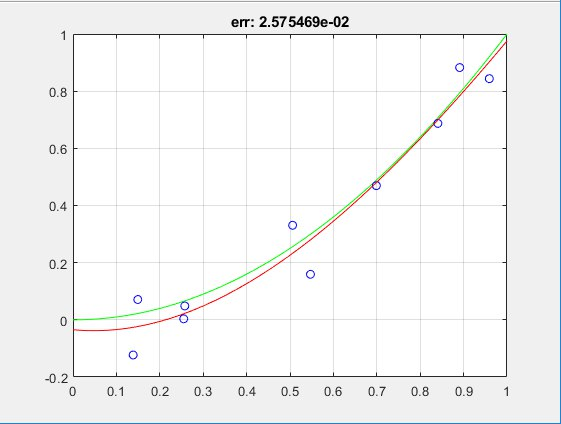
\includegraphics[width=0.5\textwidth]{regression_function.png}
	\caption{Regression Function}
	\label{fig:regression function}
\end{figure}

Figure \ref{fig:regression function} Regression function of a quadratic function

Starting from this first test, we notice that increasing the complexity of the polynomial too much produce a great loss of precision in the reconstruction.
It's therefore necessary to evaluate the variation of reconstruction, by changing $ n $ (Number of samples), $ p $ (Degree of the polynomial regressor) and $ \sigma $ (Noise variance).
So the error is calculated between $ YT $ (True function) and $ YP $ (Prediction function) and plotted in the graph. \\
Now we notice that in order to make the measurement of error more precise, it's better to repeat the experiment a sufficiently high number of times, for example, we make 30 repetitions of the prediction.

\begin{figure}[!tbp]
	\centering
	\subfloat[Error by varying n and p (from 0 to 5)]{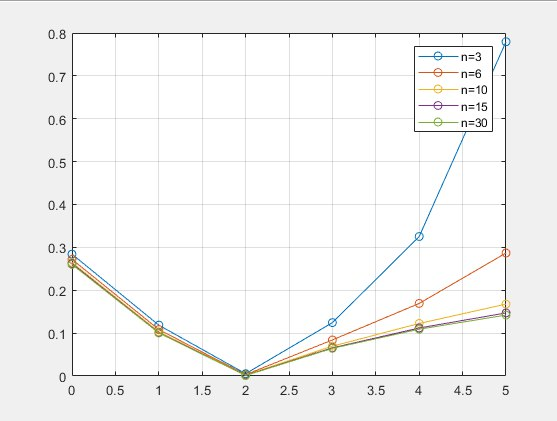
\includegraphics[width=0.45\textwidth]{error_varying_n_p.png}\label{fig:error by varying n and p}}
	\hfill
	\subfloat[Error by varying n and p (from 0 to 3)]{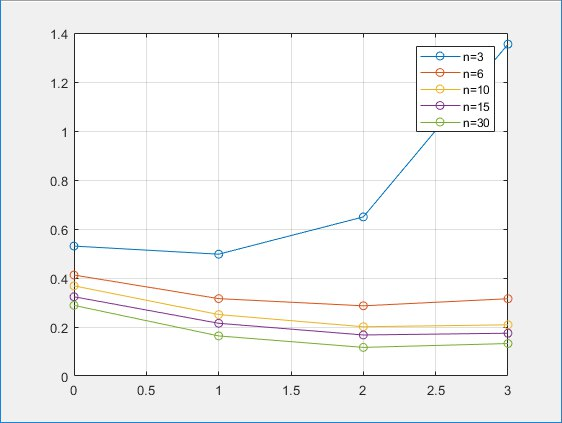
\includegraphics[width=0.45\textwidth]{error_varying_n_p2.png}\label{fig:error by varying n and p}}
	\caption{Comparing error with different values of p}
\end{figure}

\begin{figure}[!tbp]
	\centering
	\subfloat[Error by varying n and p (from 0 to 5)]{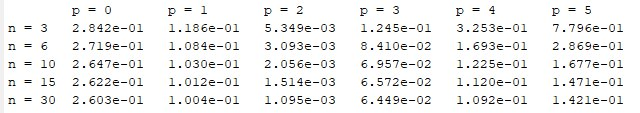
\includegraphics[width=0.5\textwidth]{table_error_varying_n_p.png}\label{fig:error by varying n and p}}
	\hfill
	\subfloat[Error by varying n and p (from 0 to 3)]{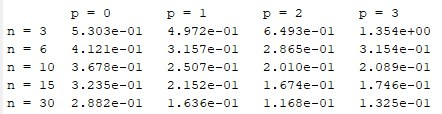
\includegraphics[width=0.4\textwidth]{table_error_varying_n_p2.png}\label{fig:error by varying n and p}}
	\caption{Comparing error with different values of p}
\end{figure}

We performed tests with some values of $ n $ and $ p $, from which it becomes clear how the error always maintains the same trend.
In particular, observing the error plots, it's evident that the maximum degree of precision is obtained for $p$ values around the degree of the original function. Obviously, using a second degree polynomial the error is minimal since the function to be reconstructed is a parabola.
Utilizing a large number of samples $n$, in general, also increases accuracy, while an increase of $p$ results in a loss of precision.
It's evident that the variation of the error between one execution of the exercise and the other is minimal for the values greater than n.
While using a small number of samples $n$, it's better to use low-grade polynomials, since an excessive number of degrees of freedom results in an attempt of the regression function to pass for each sample, making the reconstruction less precise, in particular in presence of a lot of noise, as it will try to pass for the samples even if noisy.










 
	
	\setlength\parskip{0.5cm}
	
    \chapter*{Second exercise}
    \addcontentsline{toc}{chapter}{Second exercise}
    Ripeto la regressione polinomiale dell'esercizio precedente con l'aggiunta di regolarizzatore (bias).

Con l'uso del $ bias $ $\lambda$ cerco di regolarizzare il mio polinomio: in sostanza aumetando lambda semplifico il mio risultato mentre dimunendolo utilizzo una funzione più complessa per la regressione, quindi modificare $\lambda$ è concettualmente simile a cambiare il grado del polinomio, offrendo, però, una maggior granularità nella scelta del valore ottimale.
$\lambda$ rappresenta il livello di fiducia nella qualità dei dati in ingresso: più l'ingresso è rumoroso più conviene utilizzare $\lambda$ grandi e quindi adottare soluzioni semplici in modo to not fit the noise, meno è rumoroso e più possiamo diminuire $\lambda$ ed utilizzare soluzioni più comlplesse in order to fit data.

In this exercise it's repeated the polynomial regression of the previous one with the addition of a regularizer $bias$.
With the use of $ bias $ $\lambda$ we try to regularize our polynomial: so by stretching $\lambda$ we simplify my result while using it to use a more complex function for regression, so modifying $\lambda$ is conceptually similar to changing the degree of polynomial, offering, however, a greater granularity in the choice of the optimal value.
$\lambda$ represents the level of confidence in the quality of input data: the more noisy the input, the better it's to use $\lambda$ large and then adopt simple solutions to not fit the noise, the less it is noisy and the more we can decrease $\lambda$ and use more complex solutions in order to fit data.

\begin{figure}[h]
	\centering
	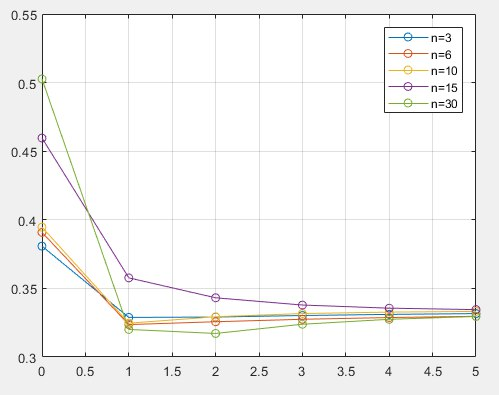
\includegraphics[width=0.5\textwidth]{pl100s10.png}
\end{figure}

\begin{figure}[h]
	\centering
	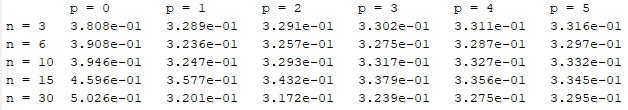
\includegraphics[width=0.5\textwidth]{tl100s10.png}
	\caption{$\lambda$ = 100 $\sigma$ = 10}
	\label{fig:lambda = 100 sigma = 10}
\end{figure}

\begin{figure}[h]
	\centering
	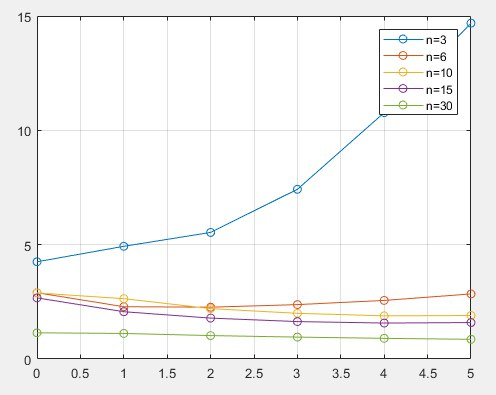
\includegraphics[width=0.5\textwidth]{pl0001s10.png}
\end{figure}

\begin{figure}[h]
	\centering
	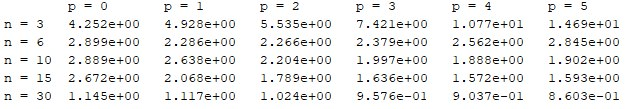
\includegraphics[width=0.5\textwidth]{tl0001s10.png}
	\caption{$\lambda$ = 0,001 $\sigma$ = 10}
	\label{fig:lambda = 0,001 sigma = 10}
\end{figure}

\begin{figure}[h]
	\centering
	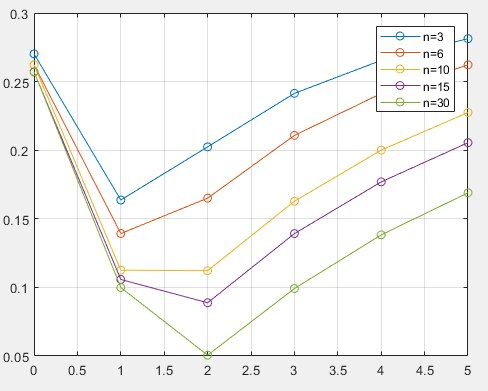
\includegraphics[width=0.5\textwidth]{pl1s001.png}
\end{figure}

\begin{figure}[h]
	\centering
	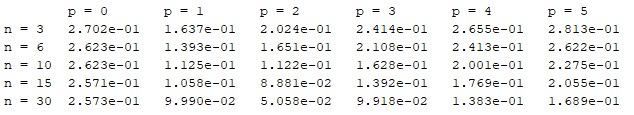
\includegraphics[width=0.5\textwidth]{tl1s001.png}
	\caption{$\lambda$ = 1 $\sigma$ = 0,01}
	\label{fig:lambda = 1 sigma = 0,01}
\end{figure}

\begin{figure}[h]
	\centering
	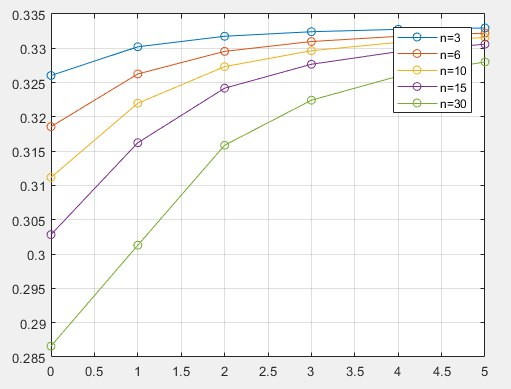
\includegraphics[width=0.5\textwidth]{pl100s01.png}
\end{figure}

\begin{figure}[h]
	\centering
	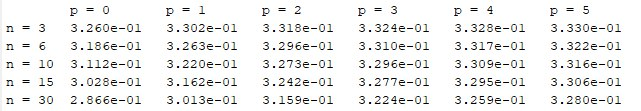
\includegraphics[width=0.5\textwidth]{tl100s01.png}
	\caption{$\lambda$ = 100 $\sigma$ = 0,01}
	\label{fig:lambda = 100 sigma = 0,01}
\end{figure}

\begin{figure}[h]
	\centering
	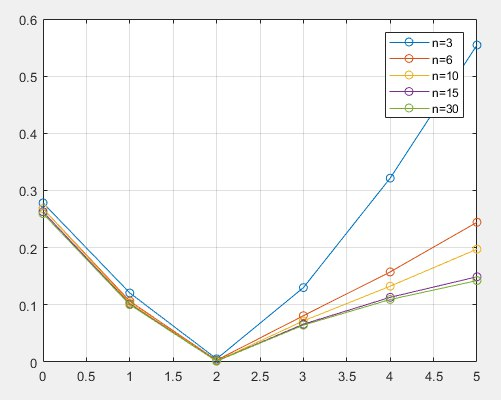
\includegraphics[width=0.5\textwidth]{pl000001s001.png}
\end{figure}

\begin{figure}[h]
	\centering
	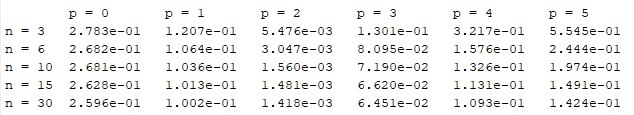
\includegraphics[width=0.5\textwidth]{tl000001s001.png}
	\caption{$\lambda$ = 0,00001 $\sigma$ = 0,01}
	\label{fig:lambda = 0,00001 sigma = 0,01}
\end{figure}
	
	\setlength\parskip{0.5cm}
	
	\chapter*{Third exercise}
	\addcontentsline{toc}{chapter}{Third exercise}
	\textbf {Kernel methods}\\

In the multidimensional case we are limited to polynomial type regressions due to the curse of dimensionality, so we use kernel methods, in particular the Gaussian kernel.\\
Use two hyperparameters:
\begin{itemize}
	\item $\lambda$ that regularize the solution $\rightarrow$ the higher it is, the more the model is flat
	\item the 3 hyperparameters of the kernel, in this case only the gamma is taken into account: a parameter that regulates the no linearity of the solution
\end{itemize}
There are combinations of $\lambda$ and $\gamma$ that more or less lead to the same solution. So $\lambda$ and $\gamma$ are parameters that are not completely disconnected, you can find more or less the same models with different values of these quantities.\\
How to find the best $\lambda$ and $\gamma$ values:\\
We find best values of hyperparmeters through validation procedure (split the data, create the model with part of the data, and test the quality of hyperparmeters on a set of data that are not used during the model creation), the best combination of hypers is the one that minimize the error on the validation set( $\rightarrow$ the set of data not used for creating the model)
The best thing to do is to mediate the results.\\
The splitting of data should not be done only once, but should be repeated because with a single report the variance is higher, but if you take the average I'm more confident that my estimator is close to the real average.\\
Observation: the loop on $k$ is put as the first loop in our implementation (putting it inside I could avoid keeping the array of all errors) because my estimate with $k$ inside would be subject to 2 types of variance: a variance due to the estimator same that can not be eliminated, the other is the variance of how the learning set and the validation set occur. Risk of selecting bad $\lambda$ and $\gamma$ because my solution is determined by the variance of the quality of the splitting. Writing the code as we wrote it, the splitting part is always the same for every $\gamma$ and $\lambda$ and this reduces the variance of my estimator.\\
Last observation: The graph, even increasing range, does not pass from all points because of the 64-bit precision that is not able to reach them all.

\begin{figure}
	\centering
	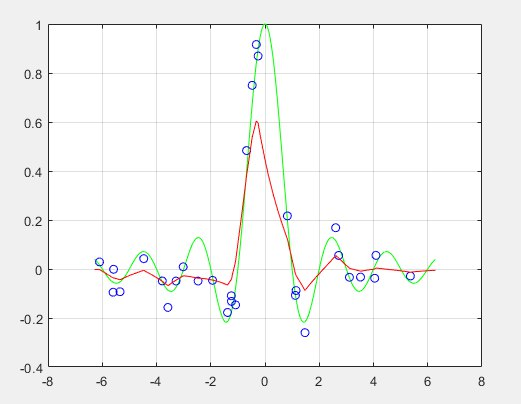
\includegraphics[width=0.5\textwidth]{kml1g1.png}
	\caption{$\lambda$ = 1 $\gamma$ = 1}
%	\label{fig:$\lambda$ = 1 $\gamma$ = 1}

\end{figure}
\begin{figure}
Less smoothness\\

	\centering
	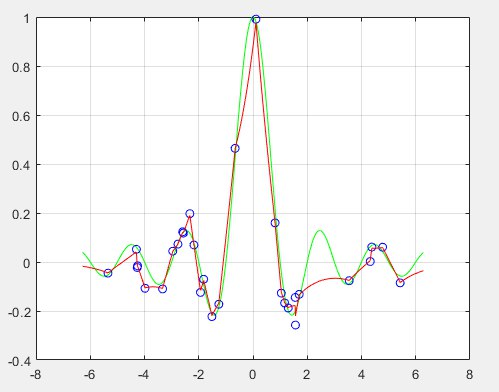
\includegraphics[width=0.5\textwidth]{kml1g001.png}
	\caption{$\lambda$ = 0,01 $\gamma$ = 1}
%	\label{fig:\lambda = 0,01 \gamma = 1}

\end{figure}
\begin{figure}
More smoothness\\

	\centering
	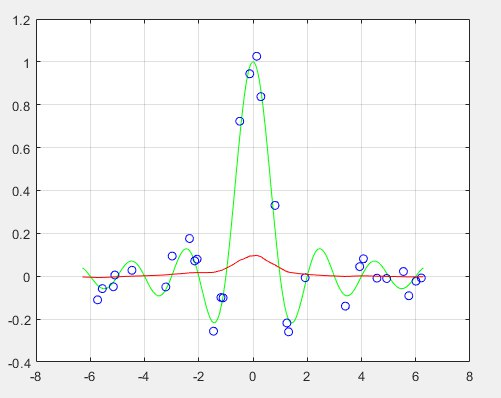
\includegraphics[width=0.5\textwidth]{kml1g25.png}
	\caption{$\lambda$ = 25 $\gamma$ = 1}
%	\label{fig:\lambda = 25 \gamma = 1}

\end{figure}
\begin{figure}
More non linearity\\

	
	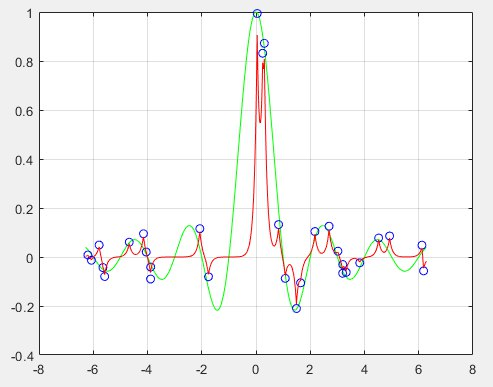
\includegraphics[width=0.5\textwidth]{kml10g01.png}
	\centering
	\caption{$\lambda$ = 0,1 $\gamma$ = 10}
%	\label{fig:\lambda = 0,1 \gamma = 10}
\end{figure}

\begin{figure}
	
Very irregular and non-linear, it can not reach all the points anyway due to the precision of the machine.\\

	
	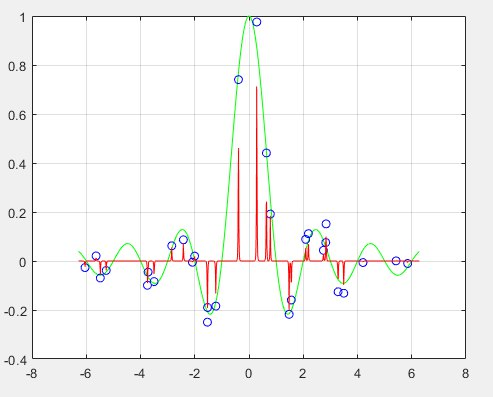
\includegraphics[width=0.5\textwidth]{kml100g0.png}
	\centering
	\caption{$\lambda$ = 0 $\gamma$ = 100}
%	\label{fig:\lambda = 0 \gamma = 100}
\end{figure}



	
	\setlength\parskip{0.5cm}
	
	\chapter*{Real World Problem}
	\addcontentsline{toc}{chapter}{Real world problem}
	We face a real-world problem as the last lab.

After understanding the problem and understanding what method use to solve it, we proceed by checking data in the dataset:
\begin{itemize}
	
	\item Categorical features
	\item Missing values
	\item Numerical problems
	
\end{itemize}
We normalize the data so that each feature has the same weight in the solution.
We control the distribution of data, checking the various categorical features that possibly have a Gaussian distribution: the Gaussian distribution indicates that data come from nature.
We observe that during the calculation two types of errors are kept:
\begin{itemize}
	
	\item Error on validation: used to optimize $\gamma$ and $\lambda$
	\item Error on the test: tells me that if we take the data and we do learning with those particular $\gamma$ and $\lambda$, we get a model with that particular unbiased error

	
\end{itemize}
To verify the goodness of model a single parameter is not enough (error for example), then we print a scatter plot: $x$ axis $\rightarrow$ true value, $y$ axis $\rightarrow$ prediction.\\
\textbf{Ideal case}: there is a line, so the values coincide exactly.\\
\textbf{Real case}: there is a bubble, an elipsoid is formed around the straight line
Using more data for learning we can improve prediction quality, so we can try to change percentages.

We note that $\lambda_{best} = 10^{-4}$ and $\gamma_{best} = 2.2122$.\\* $\lambda$ indicates the smoothness of the model and $\gamma$ indicates its non-linearity, but in itself we can not evaluate whether they are large or small.
To evaluate whether the $\gamma$ is large or small we have to evaluate the dimensionality of the space, if we are in a low-dimensional space, $\gamma = 2$ is probably large, while in one of great dimensionality it is probably small. In turn, lambda depends on the cardinality of the space, it happens that if we have small numbers in $\omega$, $\lambda$ will be large and then very regularize the solution.
In this case the size of the space is 11, so $\gamma = 2$ can be considered small.\\
\begin{figure}
We verify the distribution of the data, here for example the first categorical feature (X (:, 1)) the fact that it has a Gaussian distribution is a good sign because it is the correct distribution for data coming from nature:\\
	
	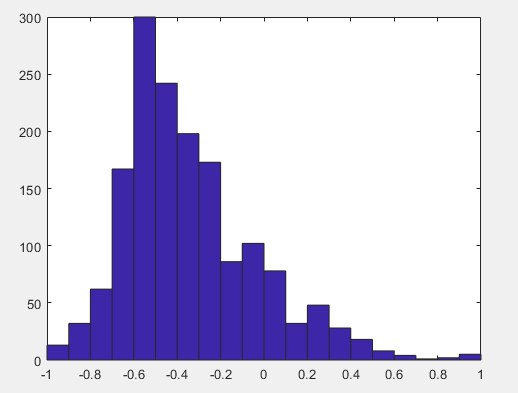
\includegraphics[width=0.5\textwidth]{hist1.png}
	\centering
	\caption{$\lambda$ = 1 $\gamma$ = 1}
	\label{fig:\lambda = 1 \gamma = 1}

	
\end{figure}

\begin{figure}

Solution with $\gamma_{best}$ and $\lambda_{best}$, values that minimize the error\\

	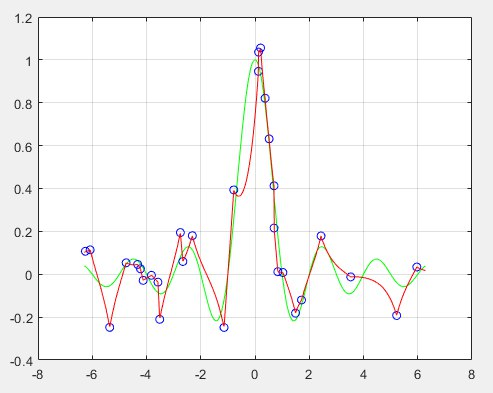
\includegraphics[width=0.5\textwidth]{kmlbgb.png}
	\centering
	\caption{$\lambda$best $\gamma$best}
%	\label{fig:\lambda_best \gamma_best}
	
	
\end{figure}

\begin{figure}
	
	We verify the distribution of data, here for example the first categorical feature (X (:, 1))
	the fact that it has a Gaussian distribution is a good sign because it is the correct distribution for data coming from nature\\
	
	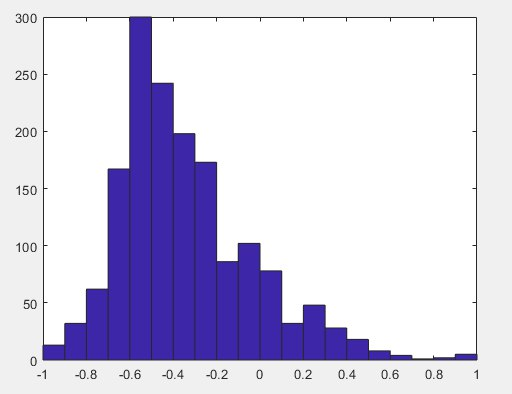
\includegraphics[width=0.5\textwidth]{hist2.png}
	\centering
	\caption{$\lambda$best $\gamma$best}
%	\label{fig:\lambda_best \gamma_best}
	
	
\end{figure}

\begin{figure}
	
	Scatter plot: x axis $\rightarrow$ true value, y axis $\rightarrow$ prediction\\
	
	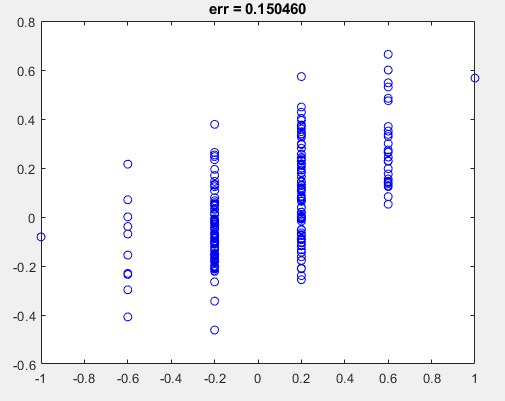
\includegraphics[width=0.5\textwidth]{scatter.png}
	\centering
	\caption{$\lambda$best $\gamma$best}
%	\label{fig:\lambda_best \gamma_best}
	
	
\end{figure}

\begin{figure}
	
	Recalculated with k = 30\\
	
	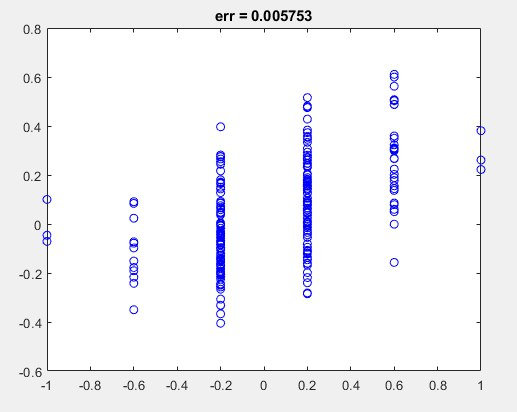
\includegraphics[width=0.5\textwidth]{scatter2.png}
	\centering
	\caption{$\lambda$best $\gamma$best}
%	\label{fig:\lambda_best \gamma_best}
	
	
\end{figure}



 
    \listoffigures

\end{document}